% !TeX document-id = {f19fb972-db1f-447e-9d78-531139c30778}
% !BIB program = biber

%\documentclass[handout]{beamer}
\documentclass[compress]{beamer}
\usepackage[T1]{fontenc}
\usetheme[block=fill,subsectionpage=progressbar,sectionpage=progressbar]{metropolis} 
\usepackage{graphicx}

\usepackage{wasysym}
\usepackage{etoolbox}
\usepackage[utf8]{inputenc}

\usepackage{pifont}

\usepackage{threeparttable}
\usepackage{subcaption}

\usepackage{tikz-qtree}
\usepackage{neuralnetwork}

\setbeamercovered{still covered={\opaqueness<1->{5}},again covered={\opaqueness<1->{100}}}


\usepackage{listings}

\lstset{
	basicstyle=\scriptsize\ttfamily,
	columns=flexible,
	breaklines=true,
	numbers=left,
	%stepsize=1,
	numberstyle=\tiny,
	backgroundcolor=\color[rgb]{0.85,0.90,1}
}



\lstnewenvironment{lstlistingoutput}{\lstset{basicstyle=\footnotesize\ttfamily,
		columns=flexible,
		breaklines=true,
		numbers=left,
		%stepsize=1,
		numberstyle=\tiny,
		backgroundcolor=\color[rgb]{.7,.7,.7}}}{}


\lstnewenvironment{lstlistingoutputtiny}{\lstset{basicstyle=\tiny\ttfamily,
		columns=flexible,
		breaklines=true,
		numbers=left,
		%stepsize=1,
		numberstyle=\tiny,
		backgroundcolor=\color[rgb]{.7,.7,.7}}}{}


% color-coded listings; replace those above 
\usepackage{xcolor}
\usepackage{minted}
\definecolor{listingbg}{rgb}{0.87,0.93,1}
\setminted[python]{
	frame=none,
	framesep=1mm,
	baselinestretch=1,
	bgcolor=listingbg,
	fontsize=\scriptsize,
	linenos,
	breaklines
	}


\usepackage[american]{babel}
\usepackage{csquotes}
\usepackage[style=apa, backend = biber]{biblatex}
\renewcommand*{\bibfont}{\tiny}


\usepackage{tikz}
\usetikzlibrary{shapes,arrows,matrix}
\usepackage{multicol}

\usepackage{subcaption}

\usepackage{booktabs}
\usepackage{graphicx}



\makeatletter
\setbeamertemplate{headline}{%
	\begin{beamercolorbox}[colsep=1.5pt]{upper separation line head}
	\end{beamercolorbox}
	\begin{beamercolorbox}{section in head/foot}
		\vskip2pt\insertnavigation{\paperwidth}\vskip2pt
	\end{beamercolorbox}%
	\begin{beamercolorbox}[colsep=1.5pt]{lower separation line head}
	\end{beamercolorbox}
}
\makeatother





\setbeamercolor{section in head/foot}{fg=normal text.bg, bg=structure.fg}


\newcommand{\instruction}[1]{\emph{\textcolor{gray}{[#1]}}}



\newcommand{\question}[1]{
	\begin{frame}[plain]
	\begin{columns}
		\column{.3\textwidth}
		\makebox[\columnwidth]{
			
\includegraphics[width=\columnwidth,height=\paperheight,keepaspectratio]{mannetje.png}}
		\column{.7\textwidth}
		\large
		\textcolor{orange}{\textbf{\emph{#1}}}
	\end{columns}
\end{frame}}


\tikzstyle{block} = [rectangle, draw, fill=blue!20, 
text width=5em, text centered, rounded corners, minimum height=4em]
\tikzstyle{line} = [draw]
\tikzstyle{pijltje} = [draw, -latex']
\tikzstyle{cloud} = [draw, ellipse,fill=red!20, node distance=3cm,
minimum height=2em, text width=4em, text centered,]


\setbeamercovered{transparent}

\addbibresource{../../resources/literature.bib}
\graphicspath{{../../resources/img/}}


\begin{document}

\title[Big Data and Automated Content Analysis]{\textbf{Big Data and Automated Content Analysis (6EC)} 
\\Week 6: »Unsupervised machine learning«
\\Monday}
\author[Anne Kroon]{Anne Kroon\\ \footnotesize{a.c.kroon@uva.nl, @annekroon \\}}
\date{May 11, 2023}
\institute[UvA CW]{UvA RM Communication Science}


\begin{frame}{}
	\titlepage
\end{frame}

\begin{frame}[standout]
Before we start: Are there questions?
\end{frame}


\begin{frame}{Today}
	\tableofcontents
\end{frame}

\section{Unsupervised machine learning}

\begin{frame}[standout]
Today: Unsupervised machine learning for text
\end{frame}

\begin{frame}{Using topic models}

	You got your model -- what now?
	
	\begin{enumerate}
	\item Assign topic scores to documents
	\item Label topics
	\item Merge topics, throw away boilerplate topics and similar (manually, or aided by cluster analysis)
	\item Compare topics between, e.g., outlets
	\item or do some time-series analysis.
	\end{enumerate}
	
	
	Example: \cite{Tsur2015}
	
	\end{frame}
	
	
	
	\subsection{Should one still use LDA?}
	
	
	\begin{frame}{The popularity of LDA}
	In the last decade, LDA has become \emph{extremely} popular in the social sciences due to
	  \begin{itemize}
	  \item easy-to-use R and Python packages
	  \item its promise to not require (a) manual (qual or quant) analysis; (b) annotations for SML; (c) creation of dictionaries etc.
	  \item a bit of a ``cool new technique'' image
	  \end{itemize}
	\end{frame}
	
	
	\begin{frame}{The popularity of LDA}
	  \textbf{But there is no silver bullet!}
	
	  Unfortunately,
	  \begin{itemize}
	  \item validating topic models is hard -- and many (most) studies don't do it (well);
	  \item there are so many choices and parameters, in combination with no simple and definite evaluation metric, that it is very hard to justify why a particular model is chosen;
	  \item experience shows that it often ``doesn't work'' $\Rightarrow$ it's quite normal to have many uninterpretable or ambigous topics;
	  \item The smaller the dataset, the less likely it is to work
	  \item LDA tends to also pick up pecularities that don't matter and outliers
	  \end{itemize}
	\end{frame}
	
	
	\begin{frame}{Solutions?}
	There are some extensions on classical LDA, in particular:
	\begin{itemize}
	\item Author-topic models
	\item Structural topic models (STM) \parencite{Roberts2014}
	\item Dynamic topic models \parencite{Blei2006}
	\end{itemize}
	
	These allow covariates (e.g., add info on who wrote a text) to improve the model, or allow to account for the changing use of words and topics over time.
	
	Also, there are techniques for validation available (e.g., topic intrusion and/or word intrusion tasks).
	\end{frame}
	
	
	\begin{frame}{Solutions?}
	  But some we can't solve everything.
	
	  \begin{itemize}
	  \item It's still BOW.
	  \item We cannot incorporate any language knowledge from larger, pre-trained datasets (e.g., via embeddings)
	  \end{itemize}
	
	$\Rightarrow$ If we think of the performance leap that we observe with Transformers in other areas, we have all reason to assume that we can do better.
	\end{frame}
	
	
	\subsection{State-of-the-art approaches to topic modelling}
	
	\begin{frame}[standout]
	Let's bring in embeddings and Transformers!
	\end{frame}
	
	
	\begin{frame}{Using embeddings and transformers for topic modelling}
	  For example:
	  \begin{itemize}[<+->]
	  \item top2vec \parencite{angelov2020top2vec}, which embeds \emph{topic vectors} in the same space as document vectors and word vectors
	  \item Contextualized Topic models \parencite{bianchi-etal-2021-pre,bianchi-etal-2021-cross}, with a lot of code examples at \url{https://contextualized-topic-models.readthedocs.io/en/latest/introduction.html}
	  \item \ldots
		\end{itemize}
	 
	\end{frame}
	
	
	
	\begin{frame}{BERTopic \parencite{Grootendorst2022}}
	%Let's discuss one specific approach: BERTtopic. 
	
	%\begin{block}{A high-level view}
	``In this paper, we introduce BERTopic, a topic model that leverages clustering techniques and a class-based variation of TF-IDF to generate coherent topic representations. More specifically, we first create document embeddings using a pretrained language model to obtain document-level information. Second, we first reduce the dimensionality of document embeddings before creating semantically similar clusters of documents that each represent a distinct topic. Third, to overcome the centroid-based perspective, we develop a classbased version of TF-IDF to extract the topic representation from each topic. These three independent steps allow for a flexible topic model that can be used in a variety of use-cases, such as dynamic topic modeling.''
	%\end{block}
	
	\tiny{(for details, read the paper)}
	
	\end{frame}
	
	
	
	
	\begin{frame}{BERTopic \parencite{Grootendorst2022}}
	  Let's look at specific examples, for instance:
	  \url{https://maartengr.github.io/BERTopic/getting_started/quickstart/quickstart.html}
	
	  but also the visualization capabilites:
	  \url{https://maartengr.github.io/BERTopic/getting_started/visualization/visualization.html#visualize-topics-per-class}
	\end{frame}
	
	
	
	
	\begin{frame}{Much more coherent topics than LDA!}
	  \makebox[\columnwidth]{	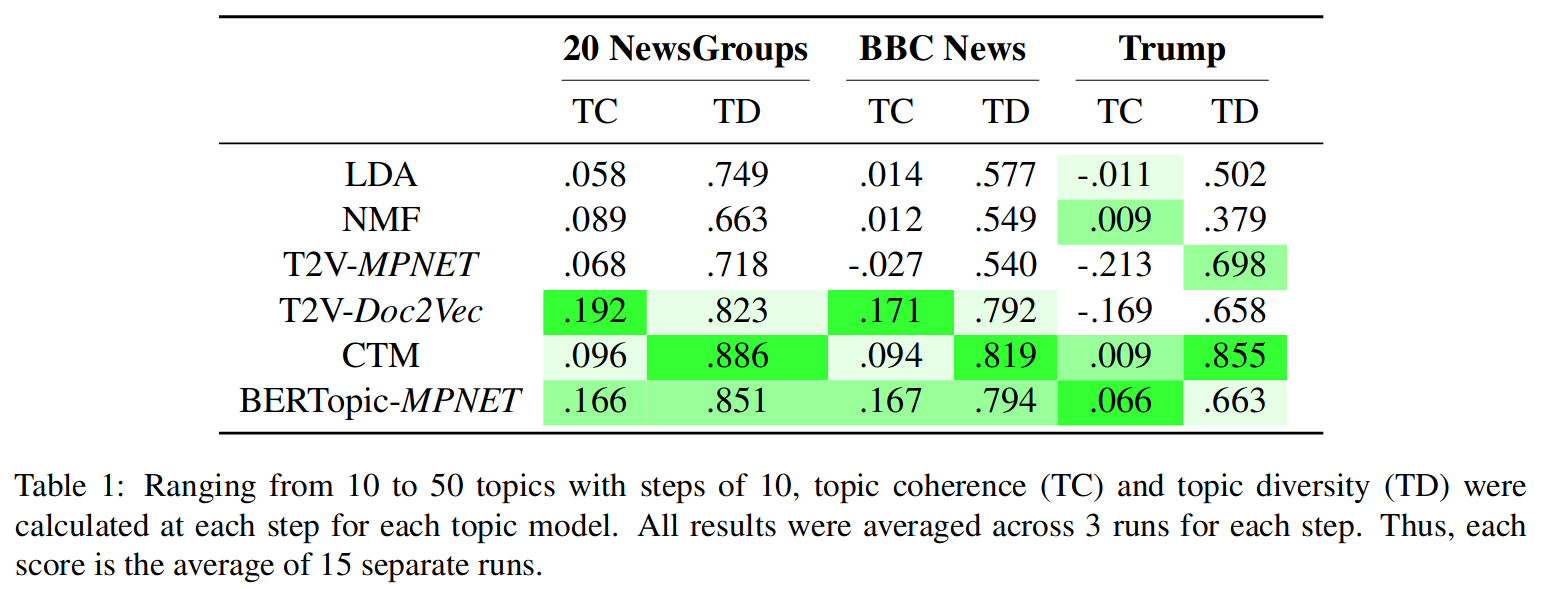
\includegraphics[width=\columnwidth,height=.8\paperheight,keepaspectratio]{grootendorst2022}}
	  (And no need to set $k$! And there is a dedicated ``outlier topic'' called $-1$!)
	\end{frame}
	
	
	\begin{frame}{Are there downsides?}
	
	  Of course!
	
	  \begin{itemize}
	  \item By definiton, much more ``black-box''-y than BOW approaches
	  \item Risk of biases introduced by LLM
	  \item Much more resource-hungry (you probably want to do this with a GPU (e.g., on CoLab)
	  \end{itemize}
	\end{frame}
	
	
	\begin{frame}[standout]
	To conclude: LDA is an interesting starting point -- but if I were to start an unsupervised topic analysis model now, I'd go for BERTopic.
	
	\end{frame}
	
	

\section{Final project}
\begin{frame}{Exercising with unsupervised machine learning for text}
Two notebooks in this week's folder: LDA and BERTopic.

But in particular, look at the BERTopic website for more examples!
\end{frame}


\begin{frame}{It's time to think about your final projects!}
\begin{itemize}
\item Let's look at the course manual!
\item Talk to me about your ideas!
\item Main point: It needs to be sth you like, and it needs to cover techniques the course!
\end{itemize}
\end{frame}

\begin{frame}[allowframebreaks,plain]
	\printbibliography
\end{frame}

\end{document}
